%% Document created 20 March 2022 automatically 
%% from /Users/massimosotgia/Desktop/uni_at_DIFI/Lab2/setup.py 

%% Copyright (C) Mattia Sotgia et al. 2022
%% Using class revtex4-2.cls
%                                       
%                                       
%██       █████  ██████         ██████  
%██      ██   ██ ██   ██             ██ 
%██      ███████ ██████          █████  
%██      ██   ██ ██   ██        ██      
%███████ ██   ██ ██████  ██     ███████ 
%                                       
%                                       
\documentclass[
    rmp,
    % preprint,
    % linenumbers,
    % tightlines,
    reprint, 
    superscriptaddress, 
    altaffilletter, 
    amsmath, 
    amssymb, 
    a4paper,
    varvw]{revtex4-2}

\usepackage[top=1.75cm,bottom=2.5cm,left=1.5cm,right=1.5cm]{geometry}

\usepackage[utf8]{inputenc}
\usepackage[T1]{fontenc}

\usepackage[italian]{babel}

%% revtex4-2 bug-fix
\def\andname{e}
%--------------------
\makeatletter
\let\it@comma@def\active@comma
\makeatother

\usepackage{txfonts}
\usepackage{graphicx}% Include figure files
\graphicspath{{../fig/}}

\usepackage{dcolumn}% Align table columns on decimal point
\usepackage{bm}% bold math
\usepackage[colorlinks, urlcolor=., bookmarks]{hyperref}% add hypertext capabilities
\renewcommand\UrlFont{\color{blue}}

\usepackage{physics}
\usepackage{siunitx}

\usepackage{fancyhdr}
\pagestyle{fancy}
\fancyhf{}
\def\twodigits#1{\ifnum#1<10 0\fi\the#1}

%-----------------------------------------------------------------------------------------------

\usepackage{background}
\SetBgColor{gray}
\SetBgAngle{90}
\SetBgScale{2}
\SetBgVshift{0.27\textwidth}

\usepackage[american resistors]{circuitikz}
\usepackage{listings}
\lstset{
  basicstyle=\fontsize{5}{6}\selectfont\ttfamily,
  % backgroundcolor=\color{white},   % choose the background color
  % basicstyle=\footnotesize,        % the size of the fonts that are used for the code
  breakatwhitespace=false,         % sets if automatic breaks should only happen at whitespace
  breaklines=true,                 % sets automatic line breaking
  captionpos=b,                    % sets the caption-position to bottom
  % commentstyle=\color{mygreen},    % comment style
  deletekeywords={...},            % if you want to delete keywords from the given language
  escapeinside={\%*}{*)},          % if you want to add LaTeX within your code
  % extendedchars=true,              % lets you use non-ASCII characters; for 8-bits encodings only, does not work with UTF-8
  % firstnumber=1000,                % start line enumeration with line 1000
  % frame=single,                    % adds a frame around the code
  % keepspaces=true,                 % keeps spaces in text, useful for keeping indentation of code (possibly needs columns=flexible). 
  % keywordstyle=\color{blue},       % keyword style
  % numbers=left,                    % where to put the line-numbers; possible values are (none, left, right)
  % numbersep=5pt,                   % how far the line-numbers are from the code
  numberstyle=\tiny\color{gray}, % the style that is used for the line-numbers
  % rulecolor=\color{black},         % if not set, the frame-color may be changed on line-breaks within not-black text (e.g. comments (green here))
  showspaces=false,                % show spaces everywhere adding particular underscores; it overrides 'showstringspaces'
  showstringspaces=false,          % underline spaces within strings only
  showtabs=false,                  % show tabs within strings adding particular underscores
  stepnumber=2,                    % the step between two line-numbers. If it's 1, each line will be numbered
  % stringstyle=\color{mymauve},     % string literal style
  tabsize=2,                       % sets default tabsize to 2 spaces
}
\usepackage{soul}


%% Define ref types
\newcommand{\reftab}[1]{Tabella {\ref{#1}}}%
\newcommand{\reffig}[1]{Figura {\ref{#1}}}%
\newcommand{\refeqn}[1]{({\ref{#1}})}%
\newcommand{\ChiSqr}{$\chi^2$\space}
\newcommand{\ChiNdf}{$\chi^2/\text{ndf}$}
\newcommand{\cernroot}{\texttt{root}}
\newcommand{\treSigma}{$3\sigma$}
\newcommand{\stdErr}[1]{$\varepsilon_{#1}$}
\newcommand{\mstdErr}[1]{\varepsilon_{#1}}
%% PAPER ONLY custom Macros

\newenvironment{methods}[1]{\section*{#1}
%\fontfamily{phv}
\fontsize{7.5}{9}\selectfont\label{sec:methods}\noindent}{\par\noindent}

%\usepackage{lcsec}

\sisetup{
    % separate-uncertainty=true,
    round-mode=uncertainty,
    % exponent-mode = scientific
}

\fancyfoot[C]{
    \the\year\twodigits\month\twodigits\day/6-\thepage
}
\fancyhead[C]{\fontfamily{phv}\fontsize{12}{12}\selectfont RELAZIONE DI LABORATORIO \textbf{
    N. 3 % ! <== CAMBIARE (Nessuna rel. -> 00)
    } (\the\year)
}

\begin{document}

\title{Misura della velocità del suono in aria
}
\thanks{Esperienza n. 6
}

\author{Francesco Polleri}
\email{s5025011@studenti.unige.it}
\author{Mattia Sotgia}
\email{s4942225@studenti.unige.it}

\collaboration{Gruppo A1}
\affiliation{Dipartimento di Fisica, Università degli Studi di Genova, I-16146 Genova, Italia}

\date{presa dati
    29 marzo--5 aprile 2022, consegnata in data 
    \today
}

\begin{abstract}
    L'esperienza è incentrata sulla costruzione e sulla caratterizzazione della logica del sistema digitale di acquisizione del dato, che permette di poter rendere la misura più rapida e più efficace, oltre che permettere di raccogliere misure in grande numero per lo stesso tipo di evento fisico, rendendo quindi possibile una trattazione statistica più efficace e corretta. Sfruttiamo poi il sistema così creato per effettuare una misura della velocità del suono in aria e confrontiamo il valore ottenuto, di \SI{347.589(669)}{\metre\per\second} con il valore teorico della velocità del suono in aria a $T=\SI{20}{\celsius}$ e $P=\SI{1}{atm}$ di \SI{343.210(338)}{\metre\per\second}, ottenendo un risultato non compatibile con la teoria, con una significatività statistica di $5.8\sigma$.
\end{abstract}

\maketitle
\thispagestyle{fancy}
% Rimuovere per consegna
\SetBgContents{
    laboratorio2: e6 [non per la consegna] \today % ! Note di versione
}


%%%% CORPO DEL TESTO
%%%% CORPO DEL TESTO


\section{Introduzione}

L'obiettivo di questa esperienza di laboratorio è effettuare una misura della velocità del suono in aria. Per ottenere tale misura sfruttiamo l'intervallo di tempo che l'onda sonora impiega a percorrere la distanza che separa l'emettitore e il ricevitore. Infatti, una volta misurato tale intervallo di tempo, è appunto necessario conoscere solamente la distanza tra i due dispositivi per ricavare la velocità del suono. Il problema principale è però ottenere una misura precisa del tempo in quanto sappiamo che l'intervalli che andiamo a misurare sono molto brevi perché il suono viaggia ad una velocità di circa \SI{340}{\metre\per\second}, per cui se posizioniamo emettitore e ricevitore ad una distanza nell'ordine delle decine di centimetri il tempo che l'onda impiega a percorrere tale distanza sarà allora nell'ordine dei millisecondi. 
Per misurare gli intervalli di tempo utilizziamo quindi due diversi metodi. Il primo metodo consiste nell'effettuare la misurazione in maniera analogica, osservando sull'oscilloscopio il ritardo temporale che intercorre tra il segnale prodotto dall'emettitore e il segnale prodotto dal ricevitore. Il secondo metodo, invece, consiste in una misura di tipo digitale. Infatti al posto di usare manualmente i cursori dell'oscilloscopio per vedere il ritardo temporale tra i due fronti d'onda, sfruttiamo una scheda Arduino DUE, che è in grado, una volta presi in input i segnali che ci interessano, di fornirci in output su un seriale i valori del ritardo temporale che appunto volevamo misurare.  

\section{Caratterizzazione apparato sperimentale analogico}\label{se:II_caratterizzazione}

Il sistema di misura è composto da un emettitore ed un ricevitore posti ad una distanza $d=[0.1, 0.5]~\si{\metre}$. Questi due strumenti, messi in comunicazione con un oscilloscopio ci permettono di misurare il ritardo tra il fronte dell'onda trasmessa e quello dell'onda ricevuta, permettendoci di individuare il ritardo tra le due onde e quindi di inferire il valore della velocità del suono in aria. 

\noindent\textit{L'emettitore.---}L'emettitore consiste in un semplice altoparlante elettronico (attuatore), caratterizzato da un diametro esterno di \SI{5.985+-0.005}{\centi\metre} capace di convertire in onde sonore un segnale elettrico che gli viene dato in ingresso. Nel nostro caso viene alimentato in ingresso da un'onda quadra, di frequenza e ampiezza variabili (in base alle necessità della misura le frequenze sono tra \SI{10}{\hertz} e \SI{10}{\kilo\hertz}). Il generatore fornisce inoltre un segnale TTL standardizzato con la stessa frequenza dell'onda in ingresso che può quindi essere utilizzato come riferimento per la misura di quest'onda.

\noindent\textit{Il ricevitore.---}Lo strumento è composto da un microfono (trasduttore) che permette di convertire in segnale analogico l'onda sonora che riceve. Il segnale analogico continuo viene poi mandato in ingresso ad un comparatore a soglia fissa\iffalse(automaticamente impostata ad un valore di \SI{00}{\volt})\fi, che quindi permette di ottenere solo due letture in uscita, un segnale alto e un segnale basso. Il segnale che quindi leggiamo dal microfono è alto se il microfono non \emph{sente} nessun suono sopra la soglia impostata con il comparatore, mentre passa ad un segnale basso appena il segnale supera la soglia. Ci interessa quindi leggere l'istante in cui il segnale passa da alto a basso, ovvero il primo fronte di discesa del segnale. 

I due strumenti sono allineati ad una guida millimetrata fissata al tavolo, necessaria per misurare la distanza tra la sorgente e il ricevitore. 

\section{Valutazione degli errori sulla misura}
\noindent\textit{Errore sulla misura della distanza.---} Lo strumento che utilizziamo per misurare la distanza è un metro caratterizzato da un errore massimo di $\SI{1}{\milli\metre}$. Poiché stiamo misurando la distanza che separa il microfono dall'altoparlante e dobbiamo quindi allineare il metro sia al punto che prendiamo come riferimento per l'emettitore, sia al punto di riferimento del ricevitore, consideriamo come errore massimo per questa misura $\SI{2}{\milli\metre}$ (consideriamo infatti \SI{1}{\milli\metre} per ogni allineamento, ipotizzando di non compiere nessun errore di parallasse), che porta quindi ad avere un errore statistico pari a $\SI{2}{\milli\metre}/\sqrt{3} = \SI{1.15}{\milli\metre}$.

\noindent\textit{Errore sulla misura del tempo.---} Per quanto riguarda l'errore sul delay nella misura analogica calcoliamo tale quantità in base a quanto è riportato sul data-sheet dell'oscilloscopio, mentre per la misura con il metodo digitale faremo una trattazione di tipo statistico, come vedremo successivamente, che ci permetterà di fornire una definizione più rigorosa degli errori statistici associati alle misure di tempo (affrontata in sezione \ref{sec:error_stat}).


\section{Presa dati \emph{analogica}}

Inizialmente utilizziamo l'oscilloscopio per effettuare misure del ritardo $t$ tra la trasmissione e la ricezione del segnale sonoro. Possiamo infatti impostare lo strumento in modo che possa fornirci una lettura di differenza temporale (delay) tra due istanti nei due segnali che forniamo in ingresso. \\
Poniamo infatti il primo cursore sul fronte di salita dell'onda quadra che genera il suono e il secondo sul primo fronte di discesa dell'onda del microfono. In questo modo lo strumento può fornire in automatico il valore di delay tra i due fronti. \\
Lasciando fisso il ricevitore spostiamo la sorgente lungo la guida e dopo aver misurato la distanza $d$ raccogliamo i valori del rispettivo ritardo per quella distanza ottenendo così una serie di coppie di valori $(t,d)$.

Ripetiamo lo stesso procedimento ponendo però uno dei due cursori non più sul primo fronte di salita dell'onda dell'emettitore, bensì sul primo fronte di discesa della stessa onda. In questo modo otteniamo un nuovo set di dati da poter confrontare con il primo. 

\noindent\textit{Scelta dei limiti sulla distanza di misura $d$.---}Le distanze a cui viene effettuata la misura sono scelte in parte per un limite fisico degli strumenti, che si traduce in una lunghezza massima della guida oltre la quale non potevamo più effettivamente misurare la distanza, e un limite invece sperimentale legato al fatto che una distanza troppo piccola non avrebbe permesso di poter distinguere l'istante di emissione e l'istante di ricezione dell'onda. Analizziamo ora nel dettaglio i due fattori limitanti nella scelta del range di distanze utilizzabili in laboratorio. 

Il primo è dovuto al funzionamento di altoparlante e microfono. Questi infatti funzionano attraverso campi elettromagnetici variabili legati alla presenza di bobine e magneti al loro interno. Perciò quando i due strumenti sono troppo vicini si possono verificare fenomeni di autoinduzione e mutua induzione. Il campo elettromagnetico derivante da questi fenomeni si propaga però alla velocità della luce, 6 ordini di grandezza maggiore della quantità che stiamo cercando di misurare, perciò l'effetto di accoppiamento emettitore-trasduttore è praticamente istantaneo, e il delay risulta essere quindi nullo. 

Un secondo effetto è legato invece alla mancanza di un vero isolamento acustico tra i due strumenti, che essendo assicurati alla stessa guida, permettono quindi la trasmissione di vibrazioni, che risultano essere trascurabili per distanze sufficientemente grandi, ma che invece possono risultare influenti a distanze molto piccole, tali per cui il suono propagato nel tavolo non si dissipa prima di raggiungere il microfono (inoltre la velocità di propagazione del suono attraverso un materiale solido risulta essere maggiore rispetto alla propagazione in aria, essendo la velocità di propagazione $v_s \propto E^{1/2}$, con $E$ modulo di Young, che risulta essere molto maggiore nei solidi rispetto all'aria ($E_\text{air}^{\SI{20}{\celsius}} = \SI{1.43e5}{\newton\per\metre\squared}$, $E_\text{solid} \geq \SI{e10}{\newton\per\metre\squared}$)\footnote{Fonte dei valori utilizzati  \url{https://www.youmath.it/lezioni/fisica/dinamica/3032-modulo-di-young.html}}). 

\section{Analisi dati \emph{analogica}}

Nell'ipotesi che la densità dell'aria sia uniforme e la temperatura costante (quindi che il valore della velocità del suono sia costante) per il tratto di spazio che l'onda sonora percorre, possiamo considerare che la velocità media $\expval{v_s}$, calcolata come distanza su tempo, sia uguale al valore istantaneo della velocità del suono $v_s$. In questa ipotesi allora la misura della velocità del suono può essere trattata al primo ordine di approssimazione come il rapporto tra una misura della distanza $d$ e una misura del tempo $t$ impiegato per coprire tale distanza. In questo modo allora otteniamo che la distanza percorsa può essere considerata come $d=v_st$, dove però stiamo ipotizzando di considerare la misura della distana in termini esatti. Ma poiché la distanza può essere considerata a meno di una costante additiva, di offset rispetto al posizionamento dell'emettitore e del ricevitore, allora è più corretto considerare una relazione \begin{equation}
    d=v_st + \delta_\text{offset}\label{eq:first_order_approx}.
\end{equation} Stiamo però ancora considerando condizioni ottimali di misura, per cui ipotizziamo che il ricevitore e l'emettitore siano perfettamente in asse, ovvero che siano allineati perfettamente anche nelle direzioni ortogonali alla trasmissione del segnale. Si potrebbe introdurre un fattore quadratico all'interno della funzione di fit che includa questo disassamento per cui la funzione risulterebbe \begin{equation}
    d=\sqrt{v_s^2t^2+2\delta_\text{offset}v_st+\qty(\delta_\text{offset}^2-\delta_\perp^2)} \label{eq:second_order_approx}
\end{equation}
Osserviamo però che questa correzione non porta a nessun cambiamento rispetto al modello lineare in quanto otteniamo che $\delta_\text{offset}^2-\delta_\perp^2 \simeq \delta_\text{offset}^2$, che porta quindi l'espressione \refeqn{eq:second_order_approx} ad essere equivalente all'espressione \refeqn{eq:first_order_approx}.

Realizziamo quindi un grafico (figura \ref{fig:analog_plot_d1}) su cui riportiamo entrambi i set di punti e facciamo un fit secondo la funzione \begin{equation}
    d(t)=v_s t+\delta_\text{offset}
\end{equation} dove $v_s$ e $\delta_\text{offset}$ sono i parametri che rappresentano rispettivamente la pendenza della retta e la sua quota, cioè, nel nostro caso, la velocità a cui ha viaggiato il suono emesso dall'altoparlante e l'offset sulla misura della distanza. Questo offset è dovuto al fatto che noi non misuriamo la distanza vera e propria tra emettitore e ricevitore perché è difficile trovare in questo modo dei punti precisi su cui prendere le misure, quindi troviamo un punto di riferimento sulla base che sostiene l'altoparlante e un punto sulla base del microfono e misuriamo la distanza tra questi. La presenza di questo offset non influisce sulla misura che vogliamo fare, in quanto la pendenza della retta, da cui ricaviamo il valore della velocità del suono, non è legata al valore dell'intercetta, purché l'offset sia lo stesso per ogni distanza a cui abbiamo preso le misure.

\begin{figure}[!t]
    \centering
    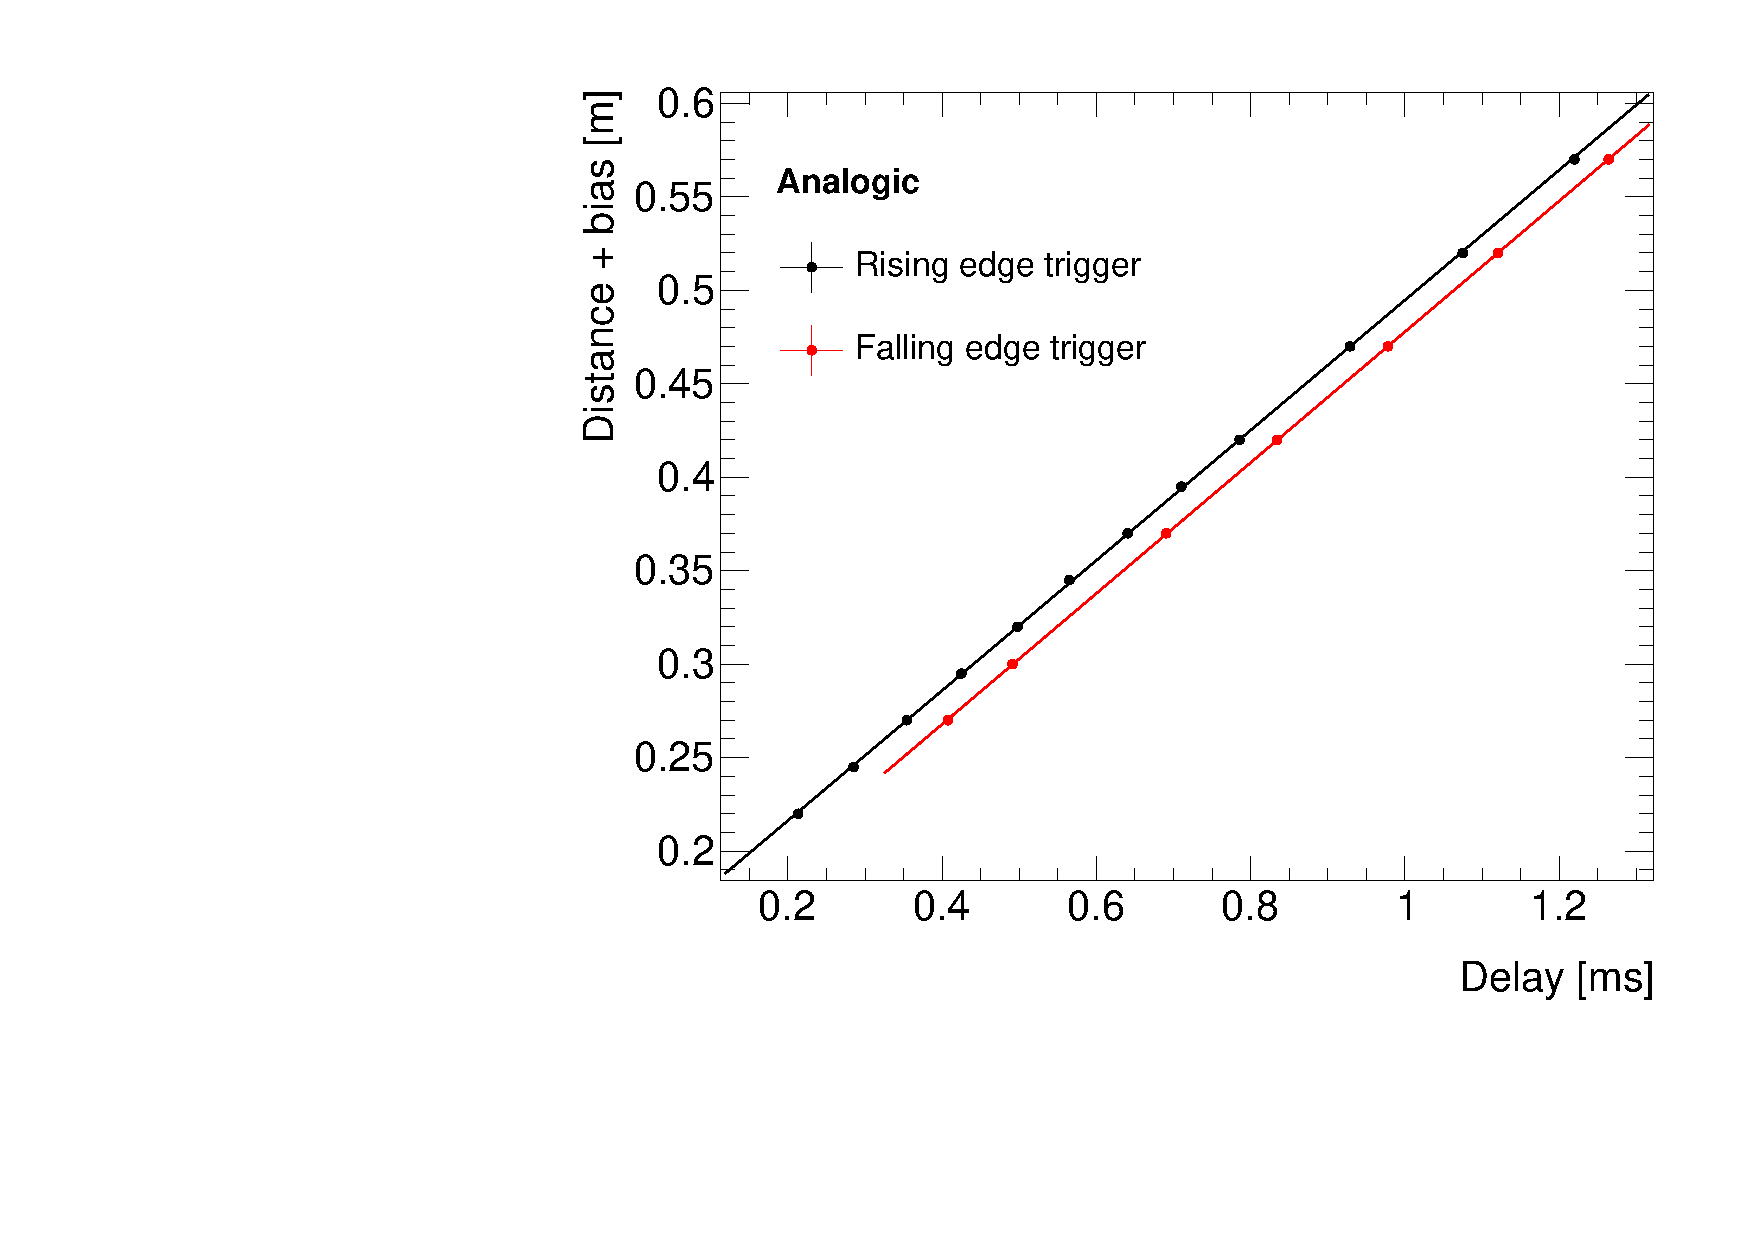
\includegraphics[width=\linewidth]{plot_analog_220417.pdf}
    \caption{Dipendenza lineare della distanza tra sorgente e ricevitore dal tempo $t$ per un'onda meccanica acustica che si propaga in aria; il coefficiente di proporzionalità esprime la velocità di propagazione $v_s$ dell'onda in aria, a pressione e temperatura di laboratorio. Possiamo osservare che esiste una differenza tra le coppie di punti acquisite considerando il fronte di salita o di discesa dell'onda quadra fornita all'emettitore, che però si risolve in una differenza di offset su tutte le misure, senza causare una differenza invece per il coefficiente di proporzionalità $v_s$.}\label{fig:analog_plot_d1}
\end{figure}

Dal fit otteniamo che, considerando i dati raccolti sfruttando l'onda prodotta sul fronte di salita del segnale emesso, \begin{align*}
    v_s &=\SI{347.77(1.16)}{\metre\per\second}\\
    \delta_\text{offset} &=\SI{0.146874(803)}{\metre},
\end{align*} mentre considerando i dati raccolti sfruttando l'onda prodotta sul fronte di discesa del segnale otteniamo \begin{align*}
    v_s &=\SI{349.85(1.65)}{\metre\per\second}\\
    \delta_\text{offset} &=\SI{0.12797(146)}{\metre}.
\end{align*}
Vediamo che i valori dei 2 offset sono nell'ordine dei centimetri, che corrisponde a ciò che ci aspettavamo, in quanto, come detto in precedenza, la distanza tra altoparlante e microfono è stata misurata usando dei punti di riferimento distanti appunto qualche centimetro dai punti in cui effettivamente veniva emesso e rivelato il suono. 

Osserviamo che i due valori del parametro $v_s$ sono compatibili (con una significatività statistica di $1.03\sigma$) e perciò possiamo ricavare la miglior stima \[v_s(\text{Analogic})=\SI{348.458(950)}{\metre\per\second}.\]

\section{Descrizione del sistema automatico di acquisizione dati}
Siccome nella misura con il metodo analogico abbiamo dovuto usare l'oscilloscopio come strumento di misura, dovendo di volta in volta riposizionare i cursori per ottenere una misura precisa del ritardo tra le due onde, vogliamo adesso trovare un modo per riuscire a raccogliere un maggior numero di dati in maniera più automatica e veloce.
Sino ad ora abbiamo misurato il ritardo temporale tra il primo fronte dell'onda quadra che permette all'altoparlante di emettere il suono e il primo fronte di discesa dell'onda del microfono, che corrisponde all'inizio dell'oscillazione della membrana del ricevitore. Sfruttando però il sistema automatico, che appunto vogliamo creare e utilizzare, possiamo rendere la misura più precisa. Possiamo infatti fare in modo che il nostro sistema acquisisca il ritardo del primo fronte di discesa e il ritardo del fronte di salita immediatamente successivo, in modo da poter fare una media e capire quale ritardo corrisponde effettivamente al massimo o minimo dell'oscillazione della membrana del microfono. Per migliorare ancora di più la precisione possiamo richiedere che il sistema acquisisca $N$ volte tali misure.

Per creare questo sistema utilizziamo una scheda Arduino DUE per la realizzazione di un timer.  Analizziamo ora la logica che permette al timer di acquisire una misura della variazione temporale dei diversi eventi misurabili. 

\noindent\textit{Routine di \emph{START} e \emph{DATA AQUISITION}.---}Quando il sistema è acceso (stato iniziale) un contatore è posto ad un conteggio zero, e il sistema è in attesa di un segnale di abilitazione, che viene fornito attraverso uno switch fisico. Fino a che lo switch non cambia il suo stato, allora il contatore è mantenuto a zero e la variabile booleana di abilitazione è impostata sul falso. Il sistema non ascolta nessun input sui canali digitali e quindi non incrementa il conteggio e non misura intervalli. Non appena l'interruttore viene cambiato, allora la scheda abilita la lettura dei segnali digitali in ingresso ed attende il passaggio del segnale dell'onda quadra sul fronte di salita per iniziare la presa dati (il sistema entra nel secondo stato accessibile, quello per cui è in attesa dei segnali digitali).

\noindent\textit{Acquisizione del singolo dato.---}Appena il segnale fornito in TTL alla scheda passa da basso ad alto (ovvero si ha un segnale di RISE per la scheda Arduino) il valore temporale in microsecondi viene salvato in memoria e appena la scheda legge sul segnale che invece arriva dal ricevitore il primo fronte di discesa e il primo fronte di salita, ne acquisisce i tempi e salva in memoria la differenza temporale tra questi due eventi e l'evento RISE sull'onda quadra. Quindi successivamente il segnale dell'onda quadra riporterà un fronte di discesa, che quindi sarà letto dalla scheda come segnale di FALL, e quindi similmente a quanto avviene per il segnale di RISE, salva il valore di tempo corrispondente a tale evento e poi misura la differenza temporale tra questo evento e i corrispondenti nuovi fronti di discesa e salita del segnale prodotto dal microfono. Questi dati vengono poi salvati in memoria. Ogni volta che un evento RISE e un evento FALL sono identificati e le relative misure effettuate, il counter interno alla scheda viene incrementato di 1. La scheda resta in attesa di una seconda coppia di eventi uguali, fino a che il counter non supera il valore $N$ prestabilito. 

\noindent\textit{Routine di \emph{STOP}.---}Quando il conteggio raggiunge il valore $N$ allora il sistema entra nel terzo stato accessibile, lo stato di fine della misura, dove i dati salvati in memoria sulla scheda sono quindi poi comunicati attraverso il seriale al computer, che immediatamente legge i relativi valori e li salva in un file. Da questo terzo stato il sistema è poi libero si ritornare allo stato iniziale di start, per cui la misura potrà dunque ricominciare da capo. 

\begin{figure*}
    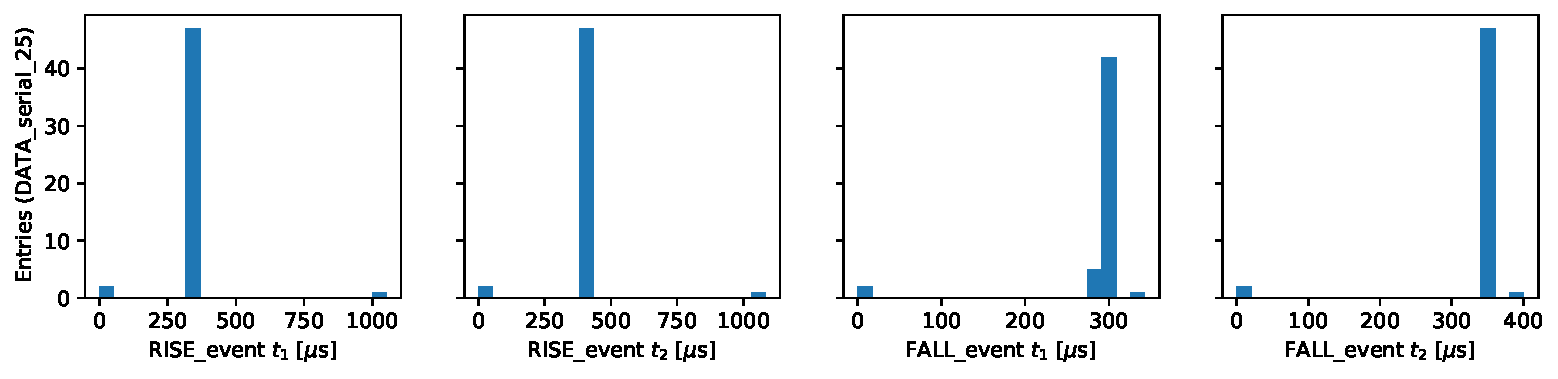
\includegraphics[width=0.85\linewidth]{histo25.pdf}
    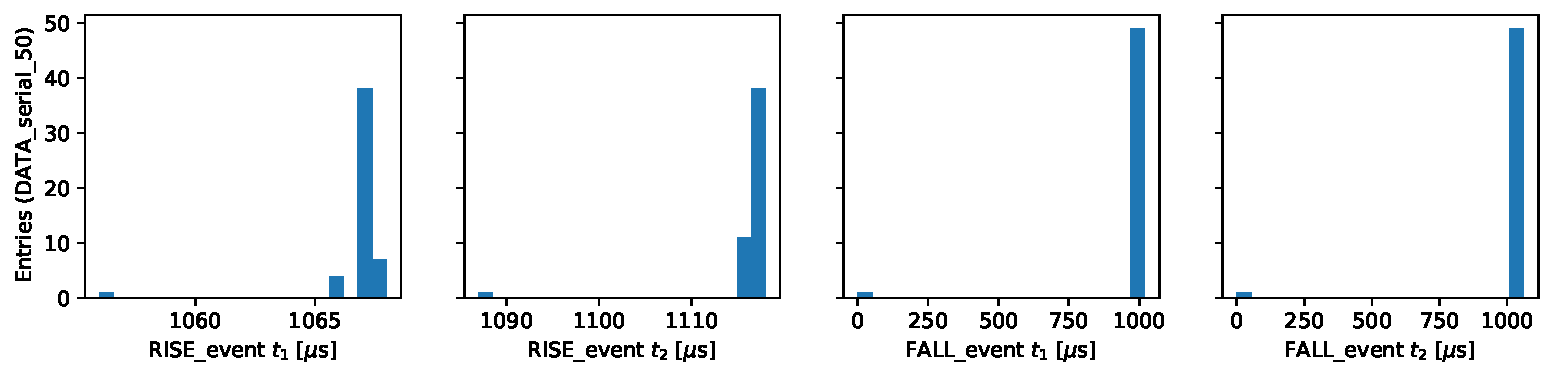
\includegraphics[width=0.85\linewidth]{histo50.pdf}
    \caption{Istogrammi dei set di dati raccolti (sono riportati quelli per le misure a \SI{0.25}{\metre} e quelle per le misure a \SI{0.5}{\metre}). Per ogni distanza sono raccolti $N=50$ punti, sia per l'evento RISE che per l'evento FALL, in due istanti differenti, un per il primo fronte di variazione del segnale fornito dal microfono, uno per il secondo fronte. La media tra queste due misure permette di ottenere poi una misura più precisa dell'effettivo fronte d'onda che viene rilevato dal microfono. }\label{fig:hists_test}
\end{figure*}

\section{Correzione degli errori di lettura del sistema}\label{sec:error_stat}
Il sistema di acquisizione così creato però potrebbe fornire in uscita dei valori di misura sbagliati, in quanto potrebbe sbagliare la lettura dei segnali sui pin digitali. Questo può essere causato da contatti elettrici non stabili o da segnali non privi di rumore, presentando quindi delle oscillazioni che possono essere interpretate dalla scheda con un evento RISE o FALL. Questo porta ad avere dei valori di delay che possono essere sbagliati, nettamente distinti e distinguibili dai valori reali medi. Possiamo infatti realizzare per ogni set di $N$ valori un istogramma e facilmente identificare i valori che possiamo definire \emph{outliers}, ovvero valori che sono nelle code delle distribuzioni dei dati raccolti. Osservando infatti un esempio di distribuzione, possiamo vedere che sono presenti dei valori di delay di \SI{0}{\micro\second} (fig. \ref{fig:hists_test} sotto, gli ultimi due istogrammi), o valori a circa \SI{1000}{\micro\second} quando il valore della media dei tempi è circa \SI{400}{\micro\second} (fig. \ref{fig:hists_test} sopra, i primi due istogrammi).
Questi punti influiscono sul valore medio e sulla deviazione standard della distribuzione in modo influente, quindi decidiamo di toglierli dal calcolo. Rimuovendo tali valori dall'insieme dei punti raccolti osserviamo che infatti gli errori associati alle misure di delay (calcolate come la deviazione standard della distribuzione dei punti, oppure posti a \SI{1}{\micro\second} se la dev. standard diventa minore della risoluzione dello strumento) diventano ragionevoli rispetto alle misure effettuate. 

\begin{figure}[!t]
    \centering
    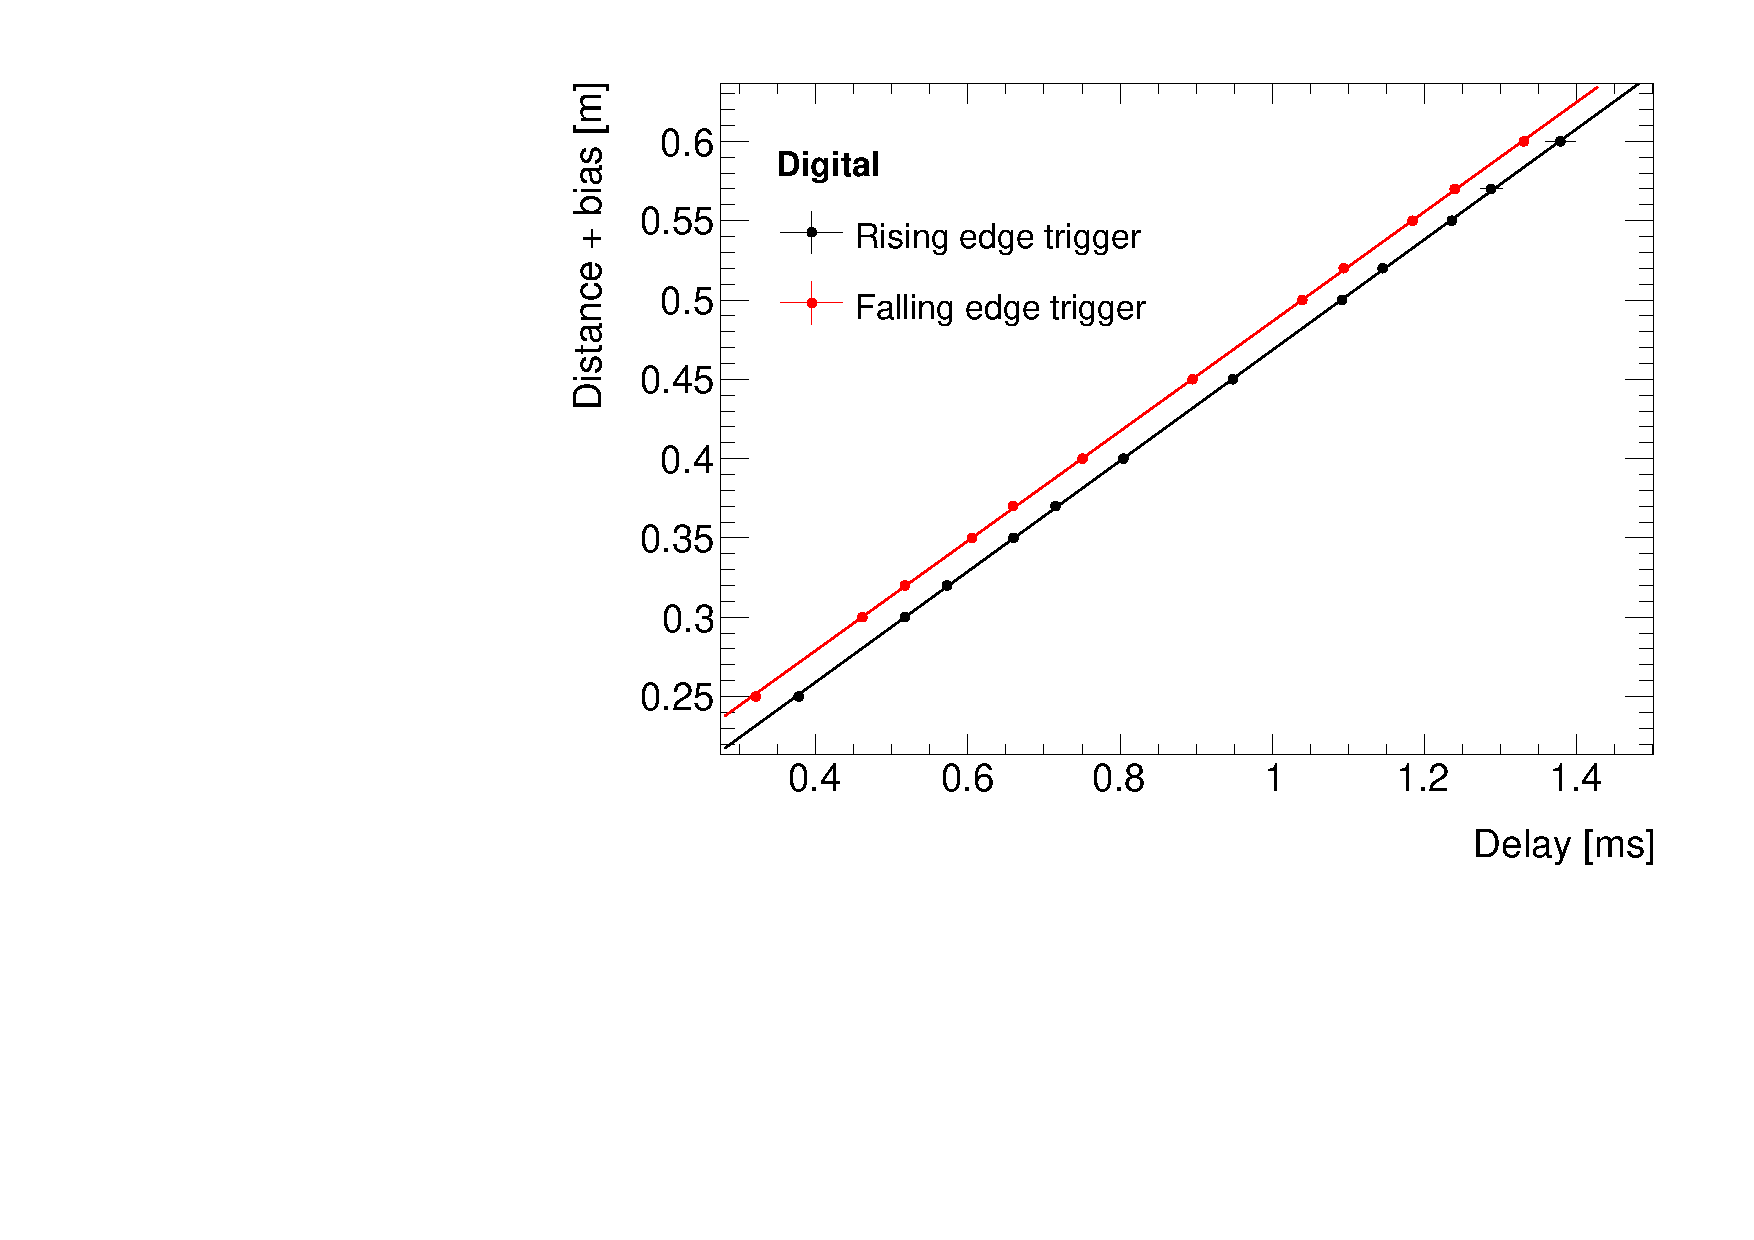
\includegraphics[width=\linewidth]{plot_digital_220417.pdf}
    \caption{Coppie di dati $(\expval{t_\text{RISE}}, d)$ e $(\expval{t_\text{FALL}}, d)$ raccolte sfruttando il sistema digitale, con i relativi fit lineari. Per entrambi i casi otteniamo che il rapporto $\chi^2/\text{ndf}$ è vicino a 1, e in entrambi i casi la Prob.($\chi^2$) è superiore al $95\%$.}\label{fig:digital_plot_d2}
\end{figure}

\section{Analisi dati, acquisizione digitale}

L'apparato sperimentale ci restituisce $N=50$ misure per ognuno dei quattro possibili delay che abbiamo deciso di misurare, questo per tutte le distanze a cui abbiamo posizionato l'altoparlante. Da questi set di dati possiamo ottenere per ogni delay un valor medio e una deviazione standard. Per ogni distanza abbiamo quindi quattro valori (ognuno con il proprio errore), due relativi al delay rispetto al fronte di salita del segnale dell'emettitore e gli altri due rispetto al fronte di discesa. Da ognuna di queste coppie possiamo ulteriormente ricavare il valor medio e una nuova deviazione standard che calcoliamo come la radice della somma in quadratura delle due deviazioni standard precedenti. Come detto in precedenza questo valor medio è quello che meglio approssima il delay corrispondente al punto in cui abbiamo il massimo o il minimo dell'oscillazione della membrana del microfono. 

Possiamo quindi riportare le coppie $(\expval{t_\text{RISE}}, d)$ e $(\expval{t_\text{FALL}}, d)$ come in figura \ref{fig:digital_plot_d2} e per ogni set di coppie realizziamo un fit secondo l'equazione (\ref{eq:first_order_approx}). Otteniamo come nel caso della misura in analogica due coppie di parametri $v_s$, $\delta_\text{offset}$.
Per gli eventi RISE troviamo quindi
\begin{align*}
    v_s &= \SI{348.48(1.43)}{\metre\per\second} \\
    \delta_\text{offset} &= \SI{0.11978(120)}{\metre}
\end{align*}
mentre per gli eventi FALL
\begin{align*}
    v_s &= \SI{345.40(1.25)}{\metre\per\second} \\
    \delta_\text{offset} &= \SI{0.14094(115)}{\metre}
\end{align*}
Otteniamo che i valori otttenuti nei due casi della velocità del suono in aria risultano essere compatibili tra di loro con una significatività statistica di $1.62\sigma$, e la miglior stima ottenuta è quindi \[v_s(\text{Digital}) = \SI{346.733(943)}{\metre\per\second}.\]


\begin{figure}
    \centering
    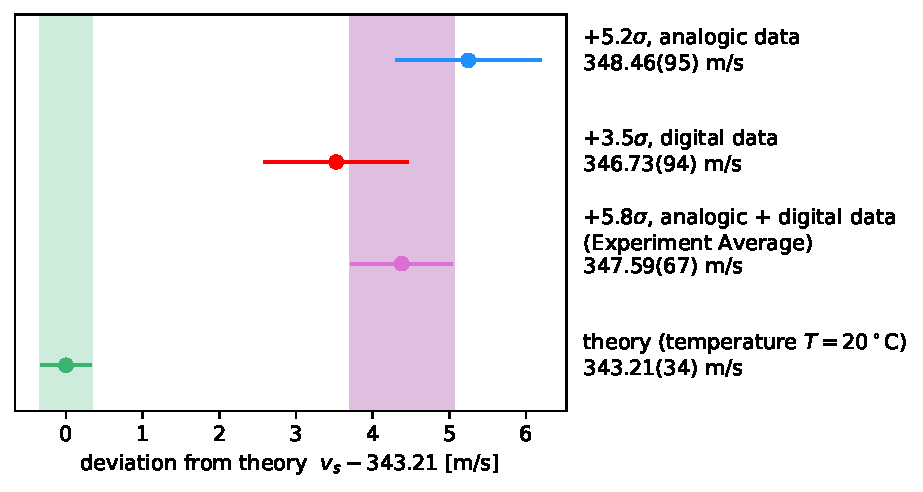
\includegraphics[width=\linewidth]{results_data_T20.pdf}
    \caption{Risultati complessivi analisi dati. Differenza sperimentale tra il valore teorico della velocità del suono \SI{343.210(338)}{\metre\per\second} e il valore misurato in laboratorio. \`E riportata anche la miglior stima del valore ottenuto in laboratorio (\SI{347.589(669)}{\metre\per\second}). Dalla figura osserviamo inoltre che il valore di $v_s(\text{Digital})$ riportato in rosso risulta essere più vicino al valore teorico (verde), rispetto a $v_s(\text{Analogic})$ (azzurro).}\label{fig:results}
\end{figure}

\iffalse
\fi

\section{Calcolo di $\vb*{v_s}$ e conclusioni}\label{sec:conclusion_compute}

Dai risultati ottenuti attraverso il metodo analogico e attraverso il metodo digitale osserviamo che i valori di $v_s(\text{Analogic})$ e $v_s(\text{Digital})$ sono compatibili con significatività statistica pari a $1.29\sigma$ per cui possiamo calcolare una miglior stima sperimentale ($v_s(\text{Exp})$), ottenendo quindi il valore \[v_s(\text{Exp}) = \SI{347.589(669)}{\metre\per\second},\] che risulta essere non compatibile con il valore teorico, con una significatività statistica di $5.8\sigma$. 

Uno dei nostri obiettivi era quello di utilizzare il metodo digitale per riuscire a fare una misura più precisa della velocità del suono. Notiamo infatti (figura \ref{fig:results}) che il valore di $v_s(\text{Digital})$ risulta essere più vicino al valore teorico della velocità del suono rispetto a quanto non lo sia il valore di $v_s(\text{Analogic})$, infatti in termini di significatività statistica il primo risulta essere di $5.2\sigma$, mentre il secondo di $3.5\sigma$. \\
Questo mette in luce quanto abbiamo detto in precedenza, ovvero che con la presa dati digitale, per cui abbiamo potuto raccogliere più dati, e anche considerare il valore medio tra i fronti di discesa e di salita dell'onda in arrivo al microfono, quindi prendendo in modo più preciso il valore del massimo (o minimo) del segnale acustico che è trasmesso sul microfono, possiamo ottenere una misura più affidabile della velocità del suono. Infatti per la presa dati analogica non abbiamo raccolto dati su entrambi i fronti, portandoci dietro quindi un possibile errore sui tempi, che ci è però difficile quantificare. \\
Questo effetto è legato al modo in cui il microfono riceve, traduce il segnale meccanico in elettrico e come poi procede a digitalizzarlo. Come infatti abbiamo già illustrato in \ref{se:II_caratterizzazione}, il microfono riceve un onda meccanica, che fa vibrare una membrana solidale ad un magnete permanente, che oscillando induce una corrente elettrica su un avvolgimento metallico. La corrente genera quindi un segnale ai capi della bobina, che viene amplificato e quindi può essere letto. Questo segnale però non è facilmente utilizzabile per effettuare una misura di ritardo temporale senza ricorrere ad una analisi dello spettro e quindi senza sfruttare strumenti matematici più \hl{fini e precisi (come le trasformate di Fourier)}. Per questo motivo ricorriamo ad un processo di digitalizzazione più semplice, facendo passare il segnale attraverso un comparatore a soglia fissata, che ci permette di avere come output dal microfono invece che un segnale continuo, un segnale discretizzato, in cui è ben visibile un salto in corrispondenza del passaggio del segnale dell'onda oltre la soglia imposta dal comparatore. \\
Prendendo in analisi un singolo segnale in arrivo al microfono, questo sarà un onda di ampiezza inizialmente nulla, che presenterà alcuni picchi in prossimità dell'arrivo del segnale e poi verrà di nuovo smorzato a zero. Ci interessiamo del primo picco, che rappresenta l'arrivo del segnale alla membrana del microfono. Questo picco produrrà una caduta di segnale e una risalita in prossimità dell'arrivo del fronte di salita dell'onda e del passaggio del fronte di discesa. La distanza tra i due eventi può variare in base all'intensità dell'onda, e quindi allargarsi e restringersi. Se quindi consideriamo solo il primo fronte per effettuare una misura del delay stiamo di fatto trascurando che l'allargamento o il restringimento di questi fronti causano uno spostamento in avanti o indietro del primo fronte, e quindi una lieve variazione nella misura del delay legata alla variazione dell'intensità dell'onda incidente sulla membrana. \\
Quindi nel caso della raccolta dati analogica, misurando solo il ritardo rispetto al primo fronte, siamo rimasti legati a questo errore sistematico. Con la presa dati digitale invece abbiamo ovviato a questo problema utilizzando non solo il valore del delay legato al primo fronte, ma considerando la media tra il primo fronte di discesa e di salita, individuando cioè il punto effettivo corrispondente al massimo o al minimo dell'onda in arrivo. Al variare dell'intensità infatti, se la larghezza del segnale aumenta, questo aumento è però simmetrico, quindi non influenza in nessun modo il punto medio. Utilizzando il punto medio come riferimento per la misura del ritardo possiamo quindi ottenere una misura più affidabile. 

Rimane comunque il problema legato al fatto che nessuno dei due valori sia compatibile con la teoria. Sembra infatti che entrambe le misure risultino spostate verso una velocità maggiore, che, ipotizzando che la strumentazione abbia funzionato in modo corretto, che l'analisi dei dati sia stata sufficientemente rigorosa e che i dati raccolti non siano affetti da errori sistematici non noti, possiamo ipotizzare sia legata ad una condizione atmosferica diversa da quella considerata per ottenere il valore teorico con cui confrontiamo i valori sperimentali (si veda l'appendice \ref{sec:appendix_A}). Possiamo quindi ipotizzare che la temperatura possa essere più alta rispetto ai \SI{20}{\celsius} considerati, e piuttosto vicina ad un valore di \SI{23}{\celsius}, per i quali i valori ottenuti potrebbero invece essere compatibili con la teoria.


\begin{methods}{D\lowercase{ati completi e codice sorgente}}
    Tutti i dati completi a supporto dei grafici, e il relativo codice, sono visualizzabili su \url{https://github.com/mattiasotgia/Lab2}. L'analisi dati viene eseguita su un programma sviluppato in C++/python basandosi su framework pubblici: ROOT, per la realizzazione dei grafici e il fit dei modelli (\url{https://root.cern/}), matplotlib, numpy e altri framework pubblici per l'analisi dei dati e la loro visualizzazione (\url{https://matplotlib.org/}, \url{https://numpy.org/}).
\end{methods}

%\onecolumngrid
\appendix

\section{Calcolo teorico della velocità del suono in aria}\label{sec:appendix_A}
Una stima teorica della velocità del suono in aria, utilizzata poi in figura \ref{fig:results} per confronto rispetto ai valori sperimentali ottenuti in laboratorio è ottenuta a partire dai valori tabulati della velocità del suono\footnote{i valori tabulati sono stati presi da \url{https://en.wikipedia.org/wiki/Speed_of_sound\#Tables}}. La temperatura nella stanza di laboratorio era di \SI{20}{\celsius} e la pressione era di \SI{1}{atm}, quindi la velocità corrispondente precisa è di \SI{343.21}{\metre\per\second}. Dalle tabelle possiamo poi anche ricavare l'incertezza associata a tale misura, considerando il valore precedente e successivo e ottenendo quindi un valore indicativo dell'errore che compiamo utilizzando questo valore tabulato della velocità. Otteniamo quindi che il valore teorico della velocità del suono in aria a $T=\SI{20}{\celsius}$ e $P=\SI{1}{atm}$ è \[v_s(\text{Theory}) = \SI{343.210(338)}{\metre\per\second},\] valore che poi possiamo confrontare con i risultati sperimentali ottenuti in laboratorio. 

\noindent\textit{Calcolo del valore teorico per $T \geq \SI{20}{\celsius}$.---}Abbiamo osservato che il valore sperimentale non si adatta perfettamente alle condizioni imposte in precedenza per il calcolo del valore teorico della velocità del suono in aria, e possiamo osservare che uno scarto di qualche \si[]{\celsius} giustificherebbe in effetti una velocità come la media sperimentale trovata in laboratorio. Possiamo quindi provare anche a ricavare dai valori tabulati anche il valore di $v_s$ per temperature differenti ($T=\SI{23}{\celsius}$, $T=\SI{25}{\celsius}$), per poi confrontarli con i valori teorici. \\
Considerando la temperatura di $T=\SI{25}{\celsius}$ direttamente dai valori in tabella possiamo ottenere \[v_s^{\SI{25}{\celsius}}(\text{Theory})=\SI{346.130(335)}{\metre\per\second}.\] 
Per il caso ad una temperatura intermedia dobbiamo invece effettuare una stima, non essendo il valore riportato in tabella, facilmente consultabile. 
Possiamo altrimenti ricavare il valore della velocità del suono in aria come funzione della temperatura, utilizzando la relazione\footnote{Questa forma può essere ricavata a partire da alcune relazioni fondamentali di carattere meccanico e termodinamico, in accordo con la teoria cinetica dei gas. Fonte \url{https://en.wikipedia.org/wiki/Speed_of_sound\#Practical_formula_for_dry_air}}\begin{equation}v_s^{air} = 331.3\sqrt{1+\frac{T^{(\si{\celsius})}}{273.15}}.~~~(\si{\metre\per\second})\end{equation} Da questa relazione possiamo quindi ottenere il valore della velocità per ogni temperatura (purché prossima alla temperatura ambiente, attorno alla quale è possibile ricavare tale relazione), ed inoltre, conoscendo l'errore sulla misura della temperatura (di circa \SI{1}{\celsius} o \SI{1}{\kelvin}) possiamo anche ricavare un valore dell'incertezza legata alla velocità del suono. 

Il valore della velocità del suono in aria ad una temperatura di $T=\SI{23}{\celsius}$ è quindi \[v_s^{\SI{23}{\celsius}}(\text{Theory})=\SI{344.9663248878187 +- 0.5824182422553077}{\metre\per\second}.\] Confrontiamo in \ref{sec:conclusion_compute} i diversi valori teorici delle velocità così ottenuti con la media sperimentale ottenuta in laboratorio. 

\setcounter{table}{0}
\renewcommand{\thetable}{A-\Roman{table}}

\end{document}
    
